\chapter*{About the author}
\addcontentsline{toc}{chapter}{About the author}

\begin{wrapfigure}{r}{0.5\textwidth}
    \vspace{-20pt}
    \begin{center}
        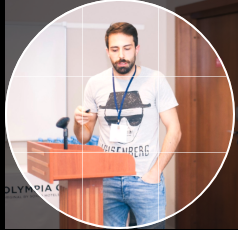
\includegraphics[width=0.48\textwidth]{images/me_linkedin}
    \end{center}
    %\vspace{-20pt}
    %\caption{A gull}
    \vspace{-15pt}
  \end{wrapfigure}

He was born the 14th February 1990 and grew up in Nicotera, a small city in Southern Italy. He attended the secondary school focusing on humanities and in 2008 he moved to Cosenza, the city where  he studied and worked for 3 years collaborating with researchers of the Department of Mathematics and Computer Science on the modellation and simulation of complex natural systems. His research interests revolve around the central topic of "Parallel Computing" in the context of High-Performance Computing (HPC). Since 2018 he lives in Eindhoven where he works as Software Engineer at ASML working on TWINSCAN photolitography systems. He studied piano and music since he was eight for ten years, long enough to make him addicted to classical and jazz music. In 2011, he obtained the Bachelor of Science in Computer Science at the University of Calabria. and since 2014 he holds the Master of Science (summa cum laude) from the University of Calabria. Since April 2015 member of the NVIDIA GPU Educational Center at UNICAL.  In  January 2018 he succesfully defended his Ph.D. thesis with title: "Acceleration of numerical regular grid methods on manycore systems".  More information on his CV.


%I am a curious and passionate software engineer and my interests include, but are not %limited to, C++, parallel programming and GPGPU. I am an active StackOverflow user, %avid reader of technical and scientific books and articles. Participating in %competitive programming competitions, writing blog articles on C++ and algorithms and %doing online
%lesson, is how I keep challenging myself daily. I feel naturally inclined to work in a %team, but I am also capable of tackling and solving complex
%problems autonomously. In addition,
%I am always looking for people and
%experiences from which I can learn
%and improve. I was born and raised in
%Nicotera, Southern Italy. At the age of
%12 I started programming and I have
%studied piano and music for 10 years,
%long enough to make me addicted
%to classical and jazz music, until the
%age of 18 when I decided to concentrate fully on Computer Science.
%Besides that, I am passionate about
%photography and investing. When I
%am not coding I am most likely either
%paddling in the Mediterranean sea,
%lifting weights in the gym or fighting
%gravity on a race bike. I drink a lot of
%coffee 
